\chapter{2D case}

\section{Problem}
In this part, we will focus on a 2D point cloud and we will use for the energy
the area of the $ r $-offset of a point cloud $ X $: the Minkowski sum with an euclidean
ball $ B(0, r) $. This offset will be denoted by $ X^r $.

\section{Area of a union of balls}
In order to compute this energy, we need to know how to estimate the area of the
intersection of a ball and a Voronoi cell. Indeed, the area of the union of
balls is the same as the sum of the areas of the restrictions of the balls to
their Voronoi cell (because the Voronoi cells partition the plane).

This is the same work as the one done in \cite{cazals2011computing} except that
we restrict ourselves to 2D which is simpler than in 3D.

For doing that, we need to decompose the intersection into triangles and
spherical caps.

The following figure illustrates the different cases for the intersection of a
Voronoi cell and a ball in 2D:
\begin{figure}[H]
    \centering
    \begin{minipage}{0.32\linewidth}
        \centering
        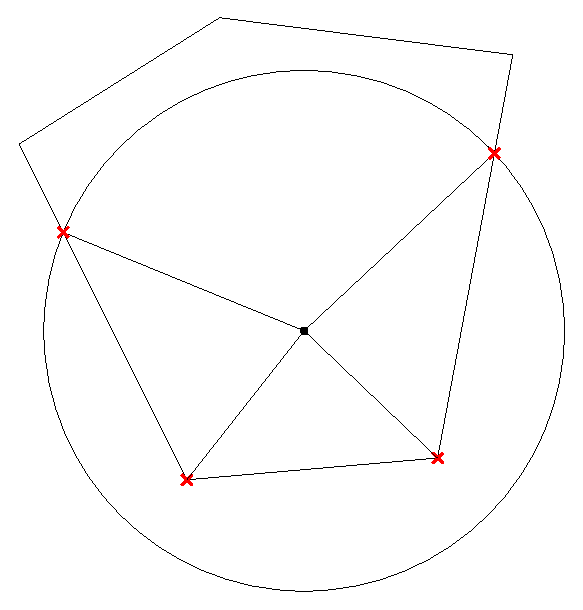
\includegraphics[scale=0.4]{2d/inter_voronoi_ball_2d}
        \subcaption{General case}
        \label{fig:inter_voronoi_ball_2d:a}
    \end{minipage}
    \begin{minipage}{0.32\linewidth}
        \centering
        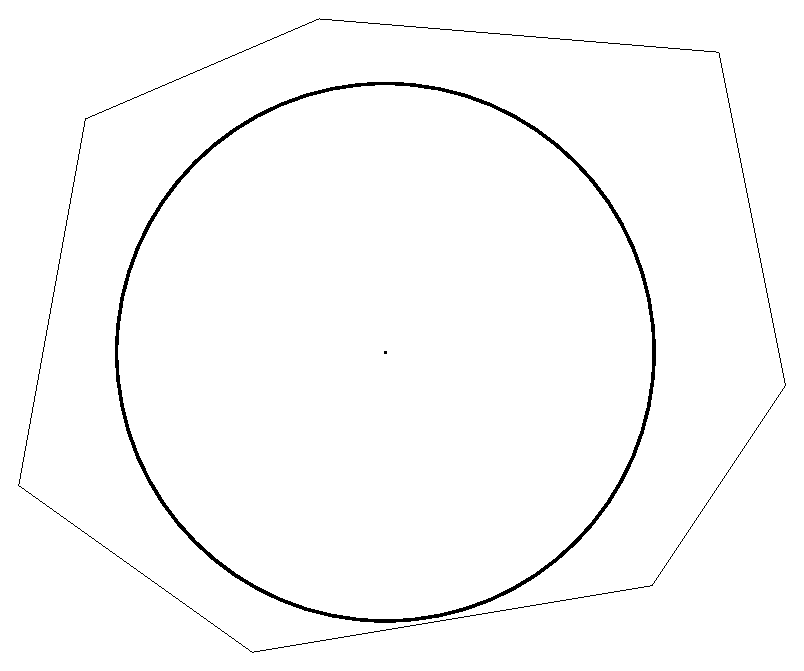
\includegraphics[scale=0.4]{2d/inter_voronoi_ball_2d_no_inter}
        \subcaption{No intersections}
        \label{fig:inter_voronoi_ball_2d:b}
    \end{minipage}
    \begin{minipage}{0.32\linewidth}
        \centering
        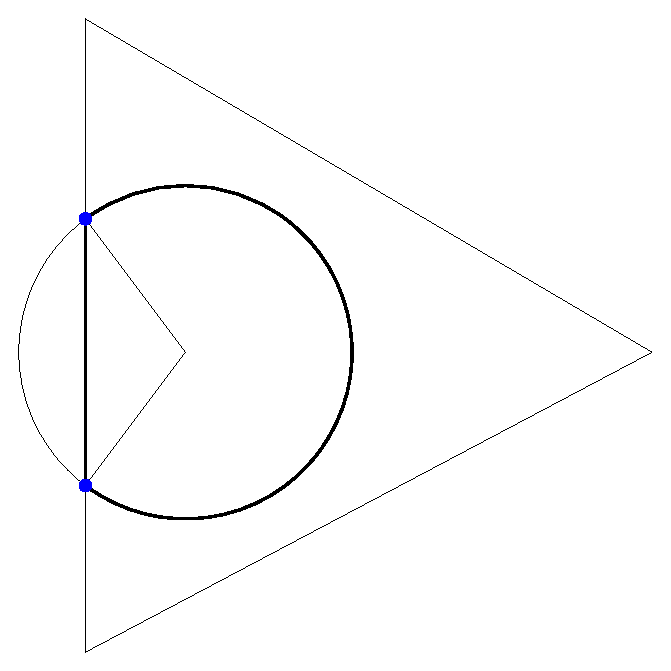
\includegraphics[scale=0.4]{2d/inter_voronoi_ball_2d_2_inter}
        \subcaption{2 intersections}
        \label{fig:inter_voronoi_ball_2d:c}
    \end{minipage}

   \caption{Different cases for the intersection between a Voronoi cell and a sphere}
   \label{fig:inter_voronoi_ball_2d}
\end{figure}

We used \texttt{CGAL} to compute the Delaunay triangulation of our point set.
Given this triangulation, we can compute the Voronoi cell of a point by doing
the following:
\begin{enumerate}
    \item Access the neighbouring faces of a vertex using the
        \texttt{incident\_faces} method.
    \item Compute the Voronoi vertices of these faces using the \texttt{dual}
        method.
\end{enumerate}

Then, we will need to know the vertices of the boundary of the intersection (the
points forming the bold boundary in \ref{fig:inter_voronoi_ball_2d}). There are
two types of those points: some are Voronoi vertices and some are intersections
of Voronoi edges and circles. To each of these points, we attach a boolean
saying whether the point is an interior point or an intersection one. We also
attach the corresponding Voronoi edge.

Then, we loop over the Voronoi edges $ e = pq $ of a vertex $ v $:
\begin{itemize}
    \item if $ p $ and $ q $ are interior points, we add the triangle $ pvq $.
    \item if $ p $ or $ q $ is interior point, we add the triangle $ pvq $.
    \item if $ p $ and $ q $ are intersection points, then if they belong to the
        same Voronoi edge, we add the triangle $ pvq $. If not, we add the
        angular sector $ \vec{vp}, \vec{vq} $.
\end{itemize}

Some special cases need to be handled:
\begin{itemize}
    \item the boundary of the Voronoi cell is entirely outside the ball, then we
        add $ \pi r^2 $ to the area of the union (see
        \ref{fig:inter_voronoi_ball_2d:b}).
    \item the boundary consists of two intersection points $ p $ and $ q $, then
        we add the triangle $ pvq $ and the angular sector $ \vec{vp}, \vec{vq}
        $ (see \ref{fig:inter_voronoi_ball_2d:c}).
    \item there is only one point on the boundary (can happen if adjacent balls
        are tangential), then we add $ \pi r^2 $.
\end{itemize}

We used the same techniques for computing the perimeter of the boundary of the
intersection except that if there are no intersection then the perimeter is null
and instead of adding triangles areas or angular sectors, we add lengths of
circular arcs.

% TODO

\section{Automatic differentiation}

The automatic differentiation is a technique used for computing the derivatives,
gradient of expressions. It is not the same as the symbolic or the numerical
differentiation.

Indeed, automatic differentiation can be used to compute derivatives of programs
and not only mathematical functions without using approximations like with
numerical differentiation.

Let us suppose that we want to compute the derivative of a function $ f $ with a
single one dimensional argument $ x $. To do that, we will replace the number
type that is to say that we will replace $ x $ by $ x + \epsilon x' $ where $
\epsilon $ with the property $ \epsilon^2 = 0 $. Then, we overload all the
arithmetical operations: addition, subtraction, multiplication, division.

Then we call $ f $ with this variable: $ f(x + \epsilon x') = y + \epsilon y'
$. We conclude that $ y = f(x) $ and $ y' = x' f'(x) $ . Indeed for small values
of $ \epsilon $, we have the first order Taylor expansion: $ f(x + \epsilon x') =
f(x) + \epsilon x' f'(x) + ... $. $ x' $ is called a seed and can be chosen
arbitrarily, we can for instance choose $ x ' = 1 $ and so $ y' = f'(x) $.

This process can be easily extended to handle functions like $ f : \R^n
\rightarrow \R $ in order to compute gradients of such functions. This is what
we did: we considered a function over $ n $ points as $ f : \R^{2n} \rightarrow
\R $.

This technique is interesting because it allows us to compute accurate
derivatives of functions very easily and efficiently. Indeed, we only have to
change the number type and write the good implementations of the basic
arithmetic operations.
In \texttt{CGAL}, this is easy to do since the library is already parametrized
by the number type.

% TODO

\section{Gradient}

Then, we used the previously described automatic differentiation technique to
compute the gradient of the previously computed area.

Here are a few examples of such gradients for different input point sets:

\begin{figure}[H]
    \centering

    \begin{minipage}{0.8\linewidth}
        \centering
        \includegraphics[scale=0.3]{2d/area/ellipse-100-01-15}
        \includegraphics[scale=0.3]{2d/area/ellipse-100-01-15-gradients}
        \subcaption{100 samples on an ellipse with $ r = 15 $}
        \label{fig:gradients_area_2d_ellipse}
    \end{minipage}

    \begin{minipage}{0.8\linewidth}
        \centering
        \includegraphics[scale=0.32]{2d/area/circle-100-01-15}
        \includegraphics[scale=0.32]{2d/area/circle-100-01-15-gradients}
        \subcaption{100 samples on a circle with $ r = 15 $}
        \label{fig:gradients_area_2d_circle}
    \end{minipage}

    \begin{minipage}{0.8\linewidth}
        \centering
        \includegraphics[scale=0.32]{2d/area/square-76-001-100}
        \includegraphics[scale=0.32]{2d/area/square-76-001-100-gradients}
        \subcaption{76 samples on a square with $ r = 100 $}
        \label{fig:gradients_area_2d_square}
    \end{minipage}

    \caption{Input point set / Computed gradients}
    \label{fig:gradients_area_2d}
\end{figure}

We did the same thing using the gradient of the perimeter of the boundary on the
same point clouds.

\begin{figure}[H]
    \centering

    \begin{minipage}{0.8\linewidth}
        \centering
        \includegraphics[scale=0.3]{2d/perimeter/ellipse-100-01-15}
        \includegraphics[scale=0.3]{2d/perimeter/ellipse-100-01-15-gradients}
        \subcaption{100 samples on an ellipse with $ r = 15 $}
        \label{fig:gradients_perimeter_2d_ellipse}
    \end{minipage}

    \begin{minipage}{0.8\linewidth}
        \centering
        \includegraphics[scale=0.32]{2d/perimeter/circle-100-01-15}
        \includegraphics[scale=0.32]{2d/perimeter/circle-100-01-15-gradients}
        \subcaption{100 samples on a circle with $ r = 15 $}
        \label{fig:gradients_perimeter_2d_circle}
    \end{minipage}

    \begin{minipage}{0.8\linewidth}
        \centering
        \includegraphics[scale=0.32]{2d/perimeter/square-76-001-100}
        \includegraphics[scale=0.32]{2d/perimeter/square-76-001-100-gradients}
        \subcaption{76 samples on a square with $ r = 100 $}
        \label{fig:gradients_perimeter_2d_square}
    \end{minipage}

    \caption{Input point set / Computed gradients}
    \label{fig:gradients_perimeter_2d}
\end{figure}

In the previous screenshots, we can see that the gradients are (if the radius of
the balls are big enough and if the sampling is sufficiently uniform) in the
same direction that the normals to the underlying surface. Also, the norm of
these gradients seem to be related to the curvature of the approximated surface.

In the next section, we will prove these two conjectures: the gradient is indeed
related to the mean curvature vector.

% TODO

\section{Relation with the mean curvature vector}

The flow we will obtain by considering the previously computed gradients will be
an approximation of the classical mean curvature flow.

Indeed, we will show that the norm of these gradients are estimations of the
mean curvature of the underlying sampled surface.

First, let's define the mean curvature vector at $ p $ of an hypersurface $ S $:
\begin{definition}
    Given an hypersurface $ S $ of $ \R^d $, the mean curvature $ \vec{\kappa}(p) $ vector at $ p
    \in S $ is defined by:
    $$ \vec{\kappa}(p) = \frac{1}{d-1} \sum_{i=1}^{d-1} \kappa_i(p) \vec{n}(p) $$
    where the $ \kappa_i(p) \in \R $ are the $ d - 1 $ principal curvatures at $ p $
    and $ \vec{n}(p) $ is the normal vector of $ S $ at $ p $.
\end{definition}

The next proposition gives the gradient of the volume of union of balls :
\begin{proposition}
    Given an hypersurface $ S $ of $ \R^d $ and points sampled on it: $ (x_i) $
    Then, if we denote by $ A $ the volume of the union of balls, then the
    partial derivatives of this quantity are:
    \begin{equation}
        \label{eqn:gradient_area_2d}
        \nabla_{x_i} A = \partiald{A}{x_i} = \int_{B} \frac{y - x_i}{||y - x_i||} dy
    \end{equation}
    where $ B = \partial B(x_i, r) \cap V(x_i, X) $.
\end{proposition}

\begin{proof}

\begin{figure}[H]
    \centering
    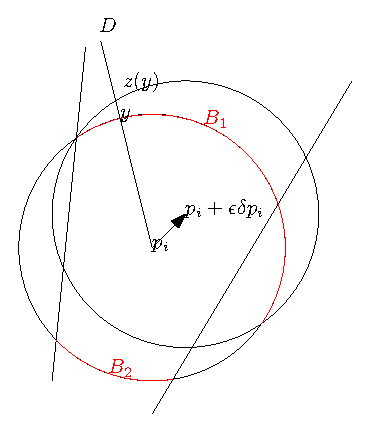
\includegraphics[scale=0.8]{2d/2d_proof_gradient_area_1}
    \caption{Situation for a ball $ B(x_i, r) $}
\end{figure}

Let's say that we move the point $ x _i $ by a small quantity $ dx_i $, let's study the variation
of the area of $ V(x_i, X) \cap B(x_i, r) $.

If we denote the old area by $ A_{old} $ and the new area by $ A_{new} $, the we
have: $ A_{new} = A_{old} + A_1 - A_2 $ where $ A_1 $ is the upper gained area
and $ A_2 $ the lower lost area.

Then, we can write that $ A_1 = \int_{B_1} || y - z(y) || dy + o(||dx_i||) $ where $ B =
\partial B(x_i, r) \cap V(x_i, X) = B_1 \cup B_2 $ is the visible boundary of
the ball.

For any $ y \in B $, we define $ z(y) $ as the intersection of the half-line $ D $
with the circle of center $ x_i + dx_i $ of radius $ r $.
Then, we parametrize the half-line $ D $ by $ y + t \frac{y - x_i}{||y - x_i||}
$ where $ t \ge 0 $.

Let's find this intersection point by assuming that $ dx_i $ and $ t $ are small
such that $ t^2 = dx_i^2 = t dx_i = o(||dx_i||^2) $.

We need to find $ D \cap C(x_i + dx_i, r) $. Let $ t \ge 0 $ then , we have :
\begin{equation}
    || y + t \frac{y - x_i}{|| y - x_i||} - (x_i + dx_i) ||^2 = r^2
    \tag{$\star$}
\end{equation}

If we expand this expression, we get:

\begin{align*}
    (\star) & \iff || y
    - (x_i + dx_i) ||^2 + t^2 + 2t \left( \frac{y-x_i}{|| y - x_i||} | y - (x_i
        + dx_i) \right) = r^2 \\
    & \iff || y - x_i || ^2 - 2 (y - x_i | dx_i) + || dx_i || ^2 + t^2 + 2t
    \left( \frac{y-x_i}{|| y - x_i||} | y - (x_i + dx_i) \right) = r^2 \\
    & \iff -2 (y - x_i | dx_i) + 2t || y - x_i|| + o(||dx_i||^2) = 0 \\
    & \iff t = t^{\star} = \left( \frac{y - x_i}{||y - x_i||} | dx_i \right) +
    o(||dx_i||)
\end{align*}

Then, $ z(y) = y + t^{\star} \frac{y - x_i}{||y - x_i||} $ and $ || y - z(y) || =
t^{\star} $.

We deduce that :
$$ A_1 = \int_{B_1} \left[ \left( \frac{y - x_i}{||y - x_i||} | dx_i \right) +
o(||dx_i||) \right] dy $$

And:

$$ A_1 - A_2 = \int_{B} \left[ \left( \frac{y - x_i}{||y - x_i||} | dx_i \right)
+ o(||dx_i||) \right] dy $$

Finally, we have, by linearity:
$$ \partiald{A}{x_i} = \int_{B} \frac{y - x_i}{||y - x_i||} dy $$

\end{proof}

Now, we will study the case where the point cloud is densely sampled on a smooth
manifold.

For this, we will need two important definitions: the $\epsilon$-sampling of a
point cloud and the reach of a manifold $ M $.

\begin{definition}
    A set of points $ x_i $ is said to be an $\epsilon$-sampling of a manifold $
    M $ if the set of the balls  $ B(x_i, \epsilon) $ verifies: $ M \subseteq
    \bigcup_i B(x_i, \epsilon) $ (see \cite{amenta1999surface}).
\end{definition}

\begin{definition}
    The reach of a manifold $ M $ denoted by $ reach(M) $ is the largest $ r
    \geq 0 $ for which for any $ p \in M^r $, there exists a unique $ q \in M $
    such that $ q = p_M(p) $ where $ p_M $ is the projection on $ M $. $ p_M(x)
    $ is defined such that $ || x - p_M(x) || = d(x, M) $.
\end{definition}

For example, if we consider a circle in the plane of radius $ R $, then every
point in the plane has a unique projection on the circle except the center which
is at distance $ R $ of every point on the circle: there is no closest point.
Consequently, its reach is $ R $.

Now, if we suppose that we have a point cloud that is an $\epsilon$-sampling of
a smooth manifold $ M $, then the following proposition gives the link between
the gradient of volume of an offset of $ M $ and the mean curvature vector.

\begin{proposition}
    Given an $\epsilon$-sampling $ P $ of a manifold $ M $ and $ r \ge 0 $ such
    that: $ \epsilon \leq r \leq reach(M) $, then:
    $$ || \nabla_p A - \vec{\kappa}(p) || \leq TODO $$
    Consequently, when $ \epsilon $ and $ \frac{\epsilon}{r} $ vanish then
    $ \nabla_p A $ converges towards the mean curvature vector of $ M $ at $ p
    $.
\end{proposition}

\begin{proof}
We will first do two approximations on \ref{eqn:gradient_area_2d}:
\begin{enumerate}
    \item the first one is to suppose that the offset of $ M $ is close enough to the offset of $ P $.
    \item the second one is that if the sampling is dense enough then we can replace $ p $
        by the projection of $ y $ on $ M $.
\end{enumerate}

Using these approximations, we get:
\begin{align*}
    \int_{\partial{P^r} \cap V(p, P)} (x - p) dx & \stackrel{(1)}{=} \int_{\partial{M^r} \cap V(p,
        P)} (x - p) dx + o(\epsilon^2) \\
    &\stackrel{(2)}{=} \int_{\partial{M^r} \cap V(p, P)} (x - p_M(x)) dx +
    o(\epsilon) \\
\end{align*}

Then, we will use the substitution $ q = p_M(x) \iff x = \phi(q) = q + \vec{n_M}(q) $
where $ \vec{n_M}(q) $ is the normal vector of $ M $ at $ q $ on the upper part
of $ \partial{M^r} \cap V(p, P) $. This substitution is a diffeomorphism because
$ r $ is smaller than the reach of $ M $.

We will need the Jacobian of this substitution. If we decompose this
substitution on $ T_p(M) \times [-r, r] $, where $ T_p(M) $ is the tangent space
of $ M $ at $ p $, we get: $ D \phi = id + r D \vec{n_M}(q) $.

Then, we use the fact that the matrix $ D \vec{n_M}(q) $ (Jacobian of the shape
operator) is diagonalizable and that its eigenvalues are the principal
curvatures.  We deduce that : $ \det (D \phi) = (1 + \kappa_1(q)) (1 +
\kappa_2(q)) $.

Using an analogous substitution on the lower part of $ \partial{M^r} \cap V(p,
P) $, we get : $ \det (D \phi) = (1 - \kappa_1(q)) (1 - \kappa_2(q)) $.

By summing the two, we obtain: $ 2 (\kappa_1(q) + \kappa_2(q)) $.

It follows that:
\begin{align*}
    \int_{\partial{M^r} \cap V(p, P)} (x - p_M(x)) dx &= \int_{M \cap V(p, P)}
    r \times \vec{n_M}(q) ( \det (id + r D \vec{n_M}(q)) - \det (id - r D
    \vec{n_M}(q)) ) dq \\
    &= 2r \int_{M \cap V(p, P)} (\kappa_1(q) + \kappa_2(q)) \vec{n_M}(q) dq \\
\end{align*}

Finally, if we suppose that $ \vec{n_M}(q) = \vec{n_M}(p) $, $ \kappa_1(q) =
\kappa_1(p) $ and $ \kappa_2(q) = \kappa_2(p) $, we have the following final
result:

$$ \nabla_p A = \partiald{A}{p} = 2r (\kappa_1(p) + \kappa_2(p)) \vec{n_M}(p) \int_{M \cap V(p, P)} dq $$

So, using the mean curvature vector:

$$ \nabla_p A = 4r \vec{\kappa}(p) Vol(M \cap V(p, P)) $$

Which means:

$$ ||\nabla_p A - \vec{\kappa}(p) || \leq | 4r Vol(M \cap V(p, P)) - 1 |
\times|| \vec{\kappa}(p) ||$$

\end{proof}

In short, the gradient of the volume of union of balls is proportional to the mean
curvature vector.

\section{Mean curvature estimation}

We can use the previous result to estimate mean curvature on a point set using
the norm of the gradients of the area of the union of balls.

We did our tests on a sampled ellipse with major / minor axes of $ a / b $. We
can parametrize this ellipse by :
$$
\begin{cases}
    x(t) &= a \cos (t) \\
    y(t) &= b \sin (t)
\end{cases}
$$

We recall the formula for computing the curvature of a parametrized curve:
$$ \kappa(t) = \frac{x'(t) y''(t) - y'(t) x''(t)}{(x'^2(t) +
    y'^2(t))^{\frac{3}{2}}} $$

For an ellipse, we obtain:
$$ \kappa(t) = \frac{ab}{(a^2 \cos^2(t) + b^2 \sin^2(t))^{\frac{3}{2}}} $$

We compare this for $ t = \frac{2 k \pi}{N} $ for $ k = 0 \ldots N - 1 $ with
the computed ones where $ N $ is the number of samples.

Here are the computed gradients mapped to a colour ramp (from green to red), we see
that the gradients are more important where the curvature is higher and are
collinear the to the outward normals.

\begin{figure}[H]
    \centering

    \includegraphics[scale=0.3]{2d/area/curvature-ellipse-200-15}
    \caption{Computed curvatures using gradients of the area with $ r = 15 $}

    \includegraphics[scale=0.3]{2d/perimeter/curvature-ellipse-200-15}
    \caption{Computed curvatures using gradients of the perimeter with $ r = 15 $}
\end{figure}

% TODO: pictures

Now, we study the absolute difference between the computed and expected
curvatures for different choices of gradients (area, perimeter of the boundary,
weighted...):

\begin{figure}[H]
    \centering

    \includegraphics[scale=0.3]{2d/area/curvature-error-ellipse-200-05}
    \caption{Error between the curvatures using gradients of the area with $ r = 0.5 $}

    \includegraphics[scale=0.3]{2d/perimeter/curvature-error-ellipse-200-05}
    \caption{Error between the curvatures using gradients of the perimeter with $ r = 0.5 $}
\end{figure}

\section{Gradient descent}

Then, as said in the introduction, we will approximate the mean curvature flow
by applying a gradient descent algorithm where the considered energy is the area
(or the perimeter of the boundary) of the union of balls.

This gradient descent will be done using a constant timestep (Euler explicit
scheme).

We needed to choose "good" weights for the gradient descent. Indeed, in a normal
mean curvature flow, all the points move with the same distance related to the
curvature. But here, this may not be the case since the energy depends on the
curvature of our restricted region.

One way to avoid this problem is to weight the gradient by the perimeter of the
visible part of the restricted region. But by doing that, we can divide by $ 0 $
so we need to choose the time step according to these weights in order to avoid
the case where a point does not see anything.

% TODO

\section{Experiments}

We did some experiments to validate our results: we first compared the two
gradient flows (area and perimeter of the boundary) to a set of points uniformly
sampled on an ellipse.

\begin{figure}[H]
    \centering

    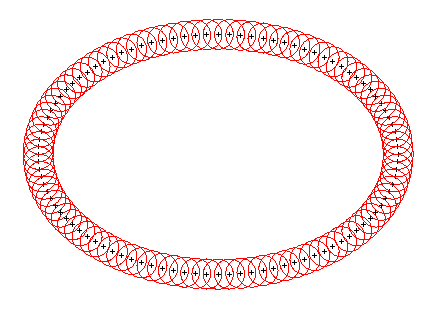
\includegraphics[scale=0.3]{2d/ellipse-balls-15}
    \subcaption{Minkowski sum of an ellipse and balls of radius $ 15 $}

    \includegraphics[scale=0.4]{2d/perimeter/ellipse-100-01-15}
    \includegraphics[scale=0.4]{2d/perimeter/ellipse-100-01-15-100}
    \subcaption{Perimeter flow : 0 / 100 iterations with a timestep of $ 0.5 $}
    \label{fig:ellipse_perimeter_flow}

    \includegraphics[scale=0.4]{2d/area/ellipse-100-01-15}
    \includegraphics[scale=0.4]{2d/area/ellipse-100-01-15-100}
    \subcaption{Area flow : 0 / 100 iterations with a timestep of $ 0.1 $}
    \label{fig:ellipse_area_flow}
\end{figure}
\vspace{-1em}
% TODO: remove extra space

Next, we add some outliers around the ellipse and observe the effects of the two
flows.

\begin{figure}[H]
    \centering

    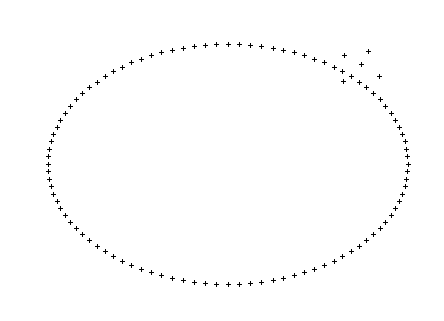
\includegraphics[scale=0.3]{2d/perimeter/ellipse-100-1-15-outliers}
    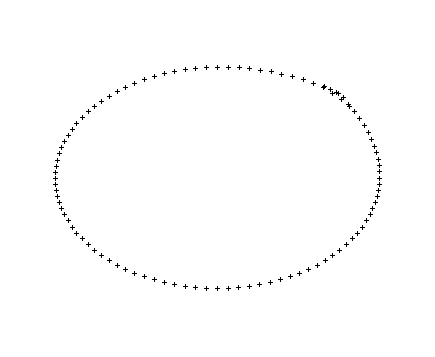
\includegraphics[scale=0.3]{2d/perimeter/ellipse-100-1-15-outliers-100}
    \subcaption{Perimeter flow : 0 / 100 iterations with a timestep of $ 1 $}
    \label{fig:ellipse_outliers_perimeter_flow}

    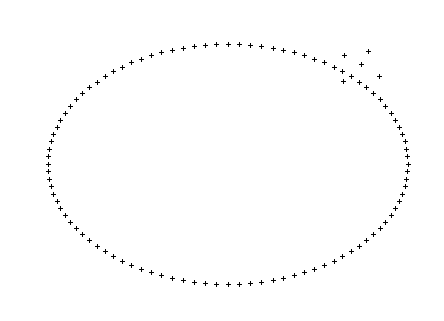
\includegraphics[scale=0.3]{2d/area/ellipse-100-01-15-outliers}
    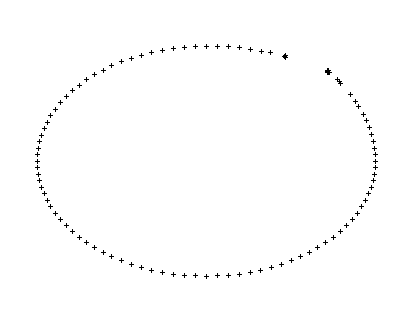
\includegraphics[scale=0.3]{2d/area/ellipse-100-01-15-outliers-40}
    \subcaption{Area flow : 0 / 40 iterations with a timestep of $ 0.1 $}
    \label{fig:ellipse_outliers_area_flow}
\end{figure}

Then, we added some Gaussian noise on these points to test the robustness of our
algorithm.

\begin{figure}[H]
    \centering

    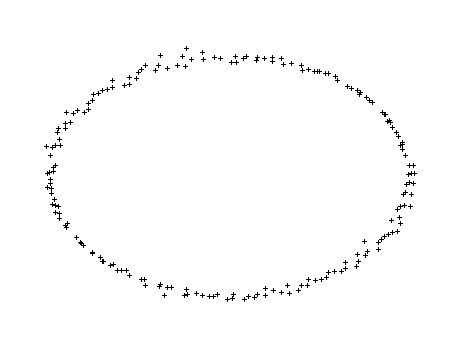
\includegraphics[scale=0.3]{2d/ellipse-noise-5-0}
    \includegraphics[scale=0.3]{2d/perimeter/ellipse-noise-5-75}
    \subcaption{Perimeter flow : 0 / 75 iterations with a timestep of $ 0.5 $}
    \label{fig:ellipse_noise_perimeter_flow}

    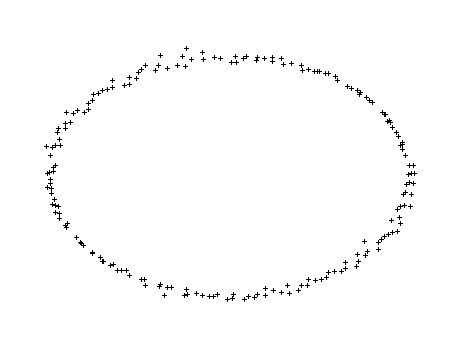
\includegraphics[scale=0.3]{2d/ellipse-noise-5-0}
    \includegraphics[scale=0.3]{2d/area/ellipse-noise-5-75}
    \subcaption{Area flow : 0 / 75 iterations with a timestep of $ 0.05 $}
    \label{fig:ellipse_noise_area_flow}
\end{figure}

We notice that the gradient flow of the area may create holes in the point set
which is not the case for the gradient flow of the perimeter.

On the contrary, the gradient flow of the perimeter of the boundary will smooth
the point set while redistributing the points in an uniform way.

% TODO: explain why
This can be explained by looking on a simple case with two intersecting balls:
\begin{itemize}
    \item for the area: TODO
    \item for the perimeter: the gradients are directed towards the outside
        and so the balls will be merged because we can say, using the triangle
        inequality, that in order to minimize the perimeter the balls must come
        closer.
\end{itemize}

The chosen radius will also influence the smoothing: points which are too far
away from other points (at distance greater than the radius) will not move. The
more the radius is big, the more points will move in big groups. Indeed, the
radius indicates how to take the neighbours of a point into account, the more
neighbours we take into account the more "global" the movement will be.

We also tried to add varying oscillations to our ellipse in order to see the
adaptive part of the algorithm. We generate oscillations with one or two
amplitudes.

For one constant amplitude:

\begin{figure}[H]
    \centering

    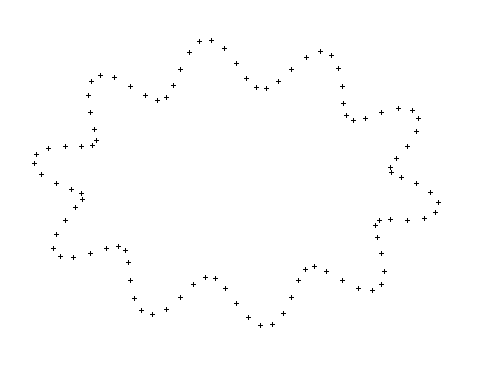
\includegraphics[scale=0.3]{2d/ellipse-osc-25-15-0}
    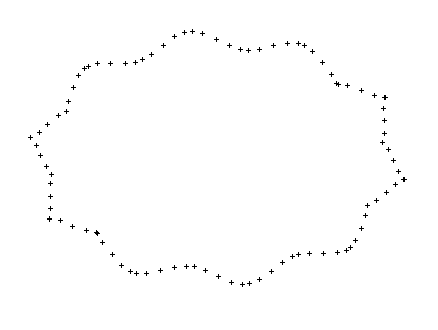
\includegraphics[scale=0.3]{2d/perimeter/ellipse-osc-25-15-50}
    \subcaption{Perimeter flow : 0 / 55 iterations with a timestep of $ 0.5 $
        and a radius of $ 15 $}
    \label{fig:ellipse_osc_perimeter_flow}

    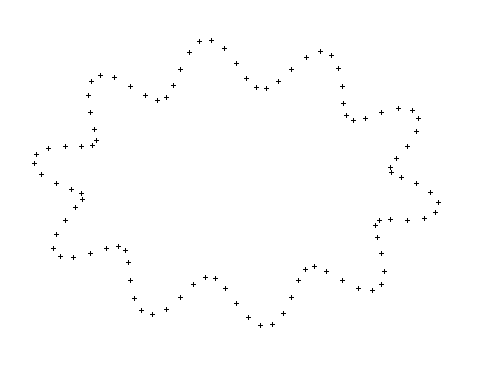
\includegraphics[scale=0.3]{2d/ellipse-osc-25-15-0}
    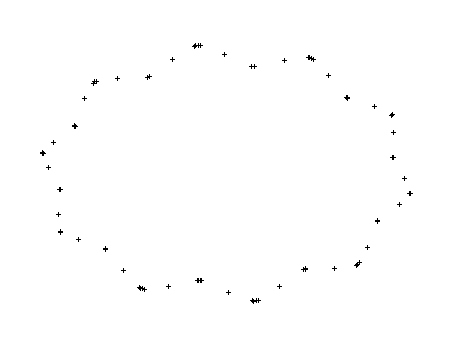
\includegraphics[scale=0.3]{2d/area/ellipse-osc-25-15-25}
    \subcaption{Area flow : 0 / 25 iterations with a timestep of $ 0.05 $ and a
        radius of $ 15 $}
    \label{fig:ellipse_osc_area_flow}
\end{figure}
% TODO: remove extra space

For two different amplitudes:

\begin{figure}[H]
    \centering

    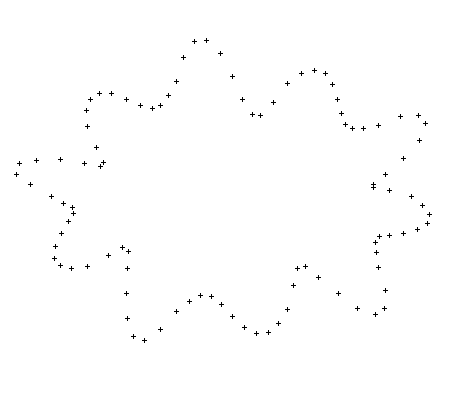
\includegraphics[scale=0.3]{2d/ellipse-osc2-20}
    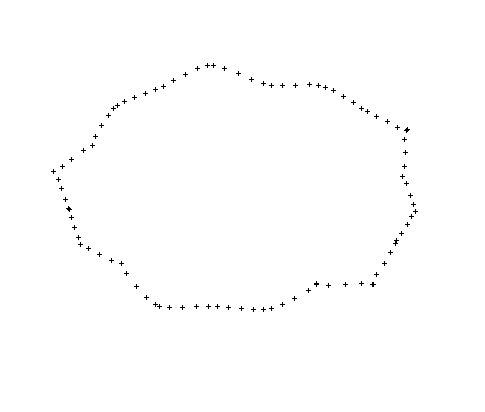
\includegraphics[scale=0.3]{2d/perimeter/ellipse-osc2-20-15-55}
    \subcaption{Perimeter flow : 0 / 55 iterations with a timestep of $ 0.5 $
        and a radius of $ 15 $}
    \label{fig:ellipse_osc2_perimeter_flow}

    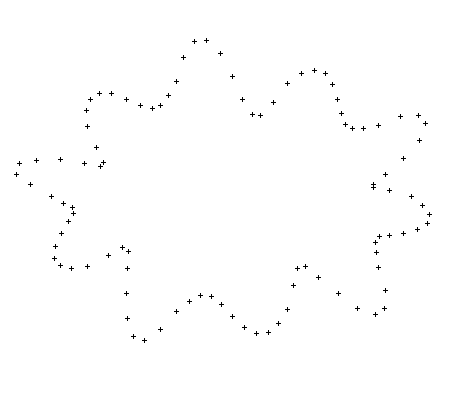
\includegraphics[scale=0.3]{2d/ellipse-osc2-20}
    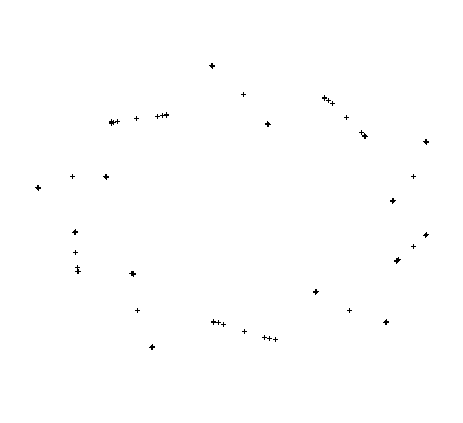
\includegraphics[scale=0.3]{2d/area/ellipse-osc2-20-15-25}
    \subcaption{Area flow : 0 / 25 iterations with a timestep of $ 0.05 $ and a
    radius of $ 15 $}
    \label{fig:ellipse_osc2_area_flow}
\end{figure}
% TODO: remove extra space

% TODO: explain why

An other experiment we did is to take points on a line segment and to fix its
endpoints. Then, we apply our flow on this point set. We expect the flow to
smooth the point set: points should get closer and closer to an uniformly
sampled set of points.

\begin{figure}[H]
    \centering

    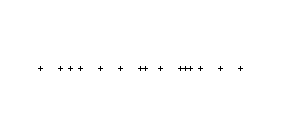
\includegraphics[scale=0.5]{2d/perimeter/line-05-15-0}
    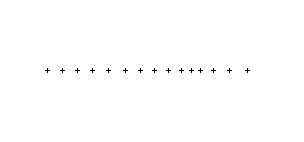
\includegraphics[scale=0.5]{2d/perimeter/line-05-15-50}
    \subcaption{Perimeter flow : 0 / 50 iterations with a timestep of $ 0.5 $}
    \label{fig:line_fixed_perimeter}

    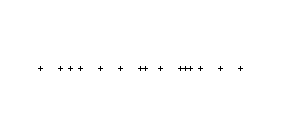
\includegraphics[scale=0.5]{2d/area/line-01-15-0}
    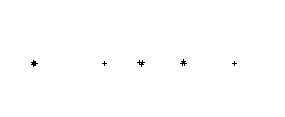
\includegraphics[scale=0.5]{2d/area/line-01-15-50}
    \subcaption{Area flow : 0 / 50 iterations with a timestep of $ 0.1 $}
    \label{fig:line_fixed_area}
\end{figure}

% TODO: explain why

\section{Assessment}

% TODO

% Union of balls
% Intersection with Voronoi cells
% Volume
% Gradient descent: weights
% Experiments

% vim: set spelllang=en :
